\section{komunikace mezi programy}\label{sec:comms}
Všechny tyto programy jsou propojeny síťovými sockety zprostředkovanými knihovnou ZeroMQ, která nabízí frontu\footnote{Ve frontě jsou zprávy seřazeny od~té nejdříve odeslané.} zpráv, bez potřeby samostatně běžícího brokeru.

Tato knihovna je~využita k~vytvoření dvou socketů, jedním lasershow přijímá příkazy od~uživatele prostřednictvím ostatních programů (vstupní socket na~portu 5557, viz obr.~\ref{fig:tcp5557}) a~do~druhého posílá informace ostatním programům (výstupní socket na~portu 5556, viz obr.~\ref{fig:tcp5556}), aby je~zprostředkovaly uživateli.
Do~prvního zmíněného posílají progamy interagující s~uživatelem příkazy pro programy lasershow a~wifi\_manager. Do~druhého posílá lasershow informace o~stavu a~změnách nastavení  a~také wifi\_manager informace o~stavu a~změnách v~nastavení WiFi.

Příkazy pro programy lasershow a~wifi\_manager vypadají následovně
\fxnote{TODO: příklady příkazů pro lasershow a~wifi\_manager z~\url{https://github.com/phuid/laser_projector/blob/master/README.md}}
\fxnote{TODO: příklady status infos od~lasershow a~wifi\_manager z~\url{https://github.com/phuid/laser_projector/blob/master/README.md}}

\begin{figure}[htb]
  \centering
  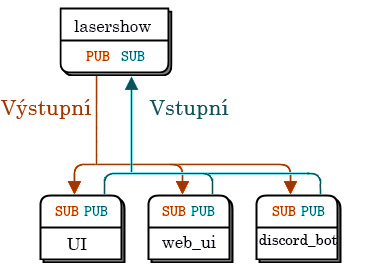
\includegraphics[width=0.5\textwidth]{img/comms_lasershow_scheme.jpg}
  \caption{\label{fig:lasershow_comms} Komunikace mezi programy vstupním socketem na~portu 5557}
\end{figure}
\begin{figure}[htb]
  \centering
  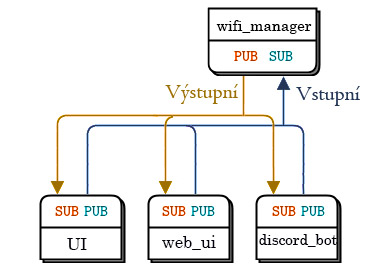
\includegraphics[width=0.5\textwidth]{img/comms_wifiman_scheme.jpg}
  \caption{\label{fig:wifiman_comms} Komunikace mezi programy výstupním socketem na~portu 5556}
\end{figure}